\documentclass[logo,reportComp]{thesis}
\usepackage[cpp,pseudo]{mypackage}

\title{数字图像处理作业一}
\subtitle{}
\school{数据科学与计算机学院}
\author{陈鸿峥}
\classname{17大数据与人工智能}
\stunum{17341015}
\headercontext{数字图像处理作业}
\lstset{language=matlab}

\begin{document}

\maketitle

本次作业包括Gamma校正及直方图均衡化两个实验。

\section{Gamma校正}
% 亮->暗 暗->亮
\subsection{原理}
对图像的每一个像素进行如下的幂次变换
\[s=cr^\gamma\]
其中$c$和$\gamma$都为正常数。
通过选取不同的$c$和$\gamma$的组合,可以实现图像的变亮或变暗操作。

\subsection{实验结果及分析}
在本实验中,$c$取$1$,$\gamma$取$0.2$和$2.5$。
从图\ref{fig:gamma0.2}中可以看出,当$\gamma<1$时,图像变亮,对比度增强,细节变得更加明显。
而从图\ref{fig:gamma2.5}中可以看出,当$\gamma>1$时,图像变暗,对比度减弱,原来亮的地方变暗了,细节也更加看不清。
\begin{figure}[H]
\centering
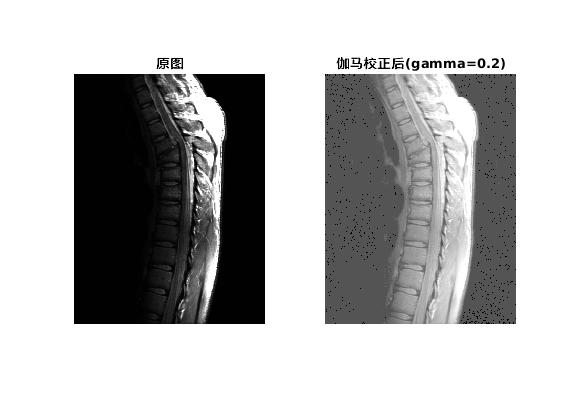
\includegraphics[width=0.8\linewidth,trim=50 80 50 50,clip]{fig/gamma02.jpg}
\caption{Gamma校正(变亮)}
\label{fig:gamma0.2}
\end{figure}
\begin{figure}[H]
\centering
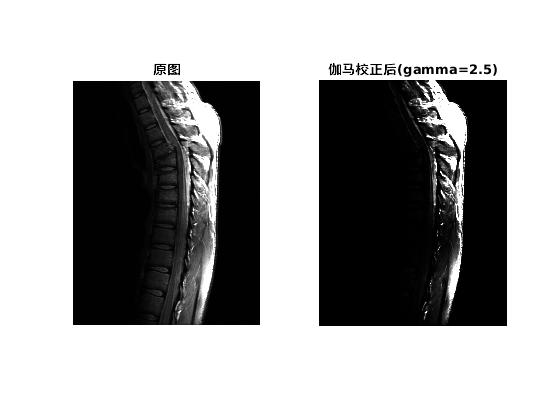
\includegraphics[width=0.8\linewidth,trim=50 80 50 50,clip]{fig/gamma25.jpg}
\caption{Gamma校正(变暗)}
\label{fig:gamma2.5}
\end{figure}

\section{直方图均衡化(PROJECT 03-02)}
% PROJECT 03-02 [Multiple Uses]
% Histogram Equalization
% (a) Write a computer program for computing the histogram of an image.
% (b) Implement the histogram equalization technique discussed in Section 3.3.1.
% (c) Download Fig. 3.8(a) and perform histogram equalization on it.
% As a minimum, your report should include the original image, a plot of its histogram, a plot of the histogram-equalization transformation function, the enhanced image, and a plot of its histogram. Use this information to explain why the resulting image was enhanced as it was.
\subsection{原理}
由于图片灰度值分布不均匀,导致图像过亮过暗,而直方图均匀化正是为了消除这种情况,使得图片细节更加容易辨认。
主要分为以下几个步骤:
\begin{itemize}
	\item 对原图片的像素进行统计,得到$[0,255]$中每一个灰度值的频数$n_k$,进而得到原图像的直方图
	\item 对原图像直方图进行归一化,由频数变为概率$p_r(r_k)=n_k/n$,实即概率质量函数(PMF)\footnote{注:由于是离散情况,故不是概率密度函数}
	\item 由概率质量函数求得累积质量函数(CMF)
	\[P(r_k)=\sum_{j=0}^kp_r(r_j)=\sum_{j=0}^k\frac{n_j}{n}\]
	\item 将原图像的灰度值作为$x$输入,从CMF中得到对应的输出值$y$,并且对$y$重新恢复尺度$[0,255]$,得到新图片中该位置的灰度值,即
	\[s_k=T(r_k)=255\cdot\sum_{j=0}^k\frac{n_j}{n}\]
	注意需要对$s_k$进行取整
	\item 对原图像中的每一个像素都这么操作,可以得到直方图归一化后的新图像
\end{itemize}

\subsection{实验结果及分析}
这里依照PROJECT 03-02的要求,选取课本的图3.8(a)进行实验。

从图\ref{fig:histogram}中可以看出,经过均衡化后的直方图分布会均衡很多,同时集中在较亮的部分。
从图\ref{fig:result}中可以看出,直方图均衡化后的图像细节更加清晰且容易辨认。
但是由于该图片本身的特性,均衡化后的直方图依然存在尖峰(某些灰度值非常多),并且均衡化后的图像存在大量噪声,这是直方图均衡化的内在缺陷。
\begin{figure}[H]
\centering
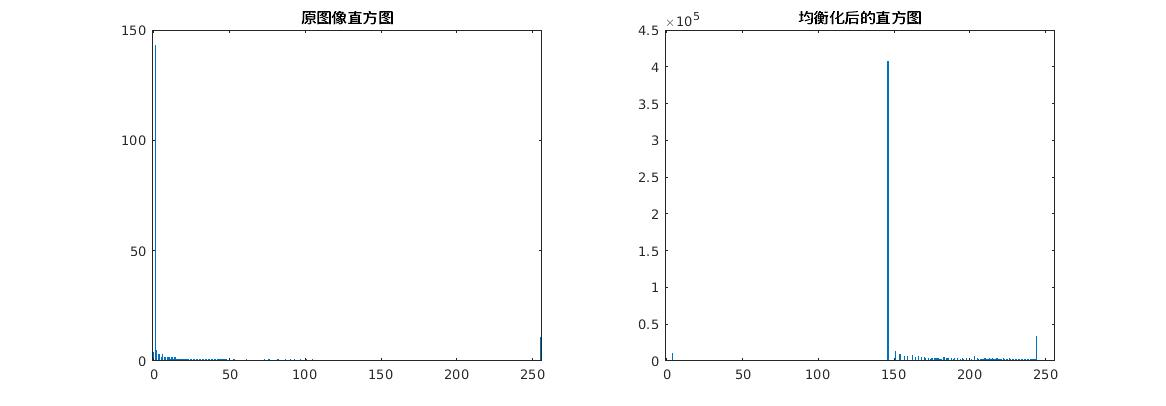
\includegraphics[width=\linewidth,trim=10 10 10 10,clip]{fig/histogram.jpg}
\caption{均衡化之前与之后的直方图}
\label{fig:histogram}
\end{figure}
\begin{figure}[H]
\centering
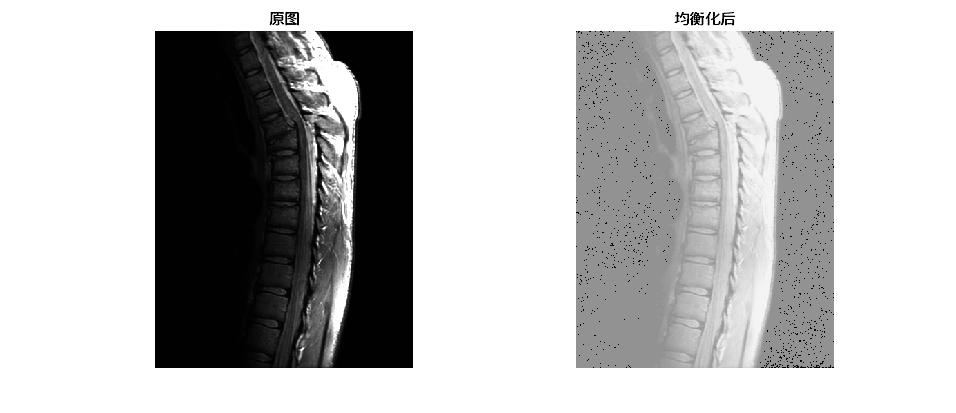
\includegraphics[width=\linewidth,trim=10 10 10 10,clip]{fig/result.jpg}
\caption{直方图均衡化结果图像}
\label{fig:result}
\end{figure}

\appendix\appendixconfig
\section{Gamma校正程序}
\begin{lstlisting}
close all;clear all;clc;
GAMMA = 2.5
I=imread('Fig0308.tif');
[m,n]=size(I);
newI=zeros(m,n);
I=double(I);
for i = 1:m
    for j = 1:n
        newI(i,j)=I(i,j).^GAMMA;
    end
end
newI=(newI-min(min(newI)))/(max(max(newI))-min(min(newI)))*255;
figure,
subplot(121),imshow(uint8(I));
title('`原图'')
subplot(122),imshow(uint8(newI));
title('`伽马校正后(gamma=2.5)'')
\end{lstlisting}

\section{直方图均衡化程序}
\begin{lstlisting}
close all;clear all;clc;
I=imread('Fig0308.tif');
[m,n]=size(I);
% J=histeq(I);
A=zeros(1,256);
for i = 1:256
    A(i)=sum(sum(I == (i-1))); % eliminate zeros
end
A=double(A);
A=A./(m*n); % normalization
cumulation=zeros(1,256);
for i = 1:256
    for j = 1:i
        cumulation(i)=cumulation(i)+A(j);
    end
end
newI=zeros(m,n);
for i = 1:m
    for j = 1:n
        newI(i,j)=uint8(cumulation(I(i,j)+1)*255);
    end
end
newA=zeros(1,256);
for i = 1:256
    newA(i)=sum(sum(newI == (i-1))); % eliminate zeros
end
figure,
subplot(121),imshow(uint8(I));
title('`原图'')
subplot(122),imshow(uint8(newI));
title('`均衡化后'')
figure,
% subplot(121),imhist(I,64);
subplot(121),bar(0:255,uint32(A*255));
title('`原图像直方图'');
% subplot(122),imhist(newI,64);
subplot(122),bar(0:255,uint32(newA));
title('`均衡化后的直方图'');
\end{lstlisting}

\end{document}

% Suggested Format for Submitting Project Reports
% Because laboratory projects are in addition to course work, it is suggested that project
% reports be kept short, and be organized in a uniform manner to simplify grading. The
% following format achieves these objectives.

% Page 1. Cover Page. Typed or printed neatly.
% · Project title
% · Project number
% · Course number
% · Student's name
% · Date due
% · Date handed in
% · Abstract (not to exceed 1/2 page)

% Page 2. Technical discussion. One to two pages (max). This section should include the
% techniques used and the principal equations (if any) implemented.

% Page 3 (or 4). Discussion of results. One to two pages (max). A discussion of results
% should include major findings in terms of the project objectives, and make clear
% reference to any images generated.

% Results. Includes all the images generated in the project. Number images individually
% so they can be referenced in the preceding discussions.

% Appendix. Program listings. Includes listings of all programs written by the student.
% Standard routines and other material obtained from other sources should be
% acknowledged by name, but their listings should not be included.

% Layout. The entire report must be in standard sheet size format (8.5 x 11 inches in the
% U.S.) All sheets should be stapled in three locations to form a binding booklet-like
% support on the left margin. Alternatively, sheets can be assembled using a commercial
% plastic binding product with a clear plastic cover.

% A note on program implementation: As noted earlier, the objective of the computer
% programs used in the following projects is to teach the student how to manipulate
% images. There are numerous packages that perform some of the functions required to
% implement the projects. However, the use of "canned" routines as the only method to
% implement an entire project is discouraged. For example, if the students are using
% MATLAB and the Image Processing Toolbox, a balanced approach is to use MATLAB's
% programming environment to write M functions to implement the projects, using some of
% MATLAB's own functions in the process. A good example is the implementation of the 2-
% D Fourier Fast Transform. The student should use the MATLAB function that computes
% the 2-D FFT directly, but write functions for operations such as centering the transform,
% multiplying it by a filter function, and obtaining the spectrum.